\documentclass[12pt,a4paper]{article}
\usepackage[utf8]{inputenc}
\usepackage[spanish]{babel}
\usepackage{geometry}
\usepackage{graphicx}
\usepackage{booktabs}
\usepackage{amsmath}
\usepackage{hyperref}
\usepackage{float}
\usepackage{subcaption}
\usepackage{listings}
\usepackage{xcolor}
\usepackage{amssymb}  % Para símbolos como \checkmark

\geometry{margin=2.5cm}

\hypersetup{
    colorlinks=true,
    linkcolor=blue,
    filecolor=magenta,
    urlcolor=cyan,
}

\lstset{
    basicstyle=\ttfamily\small,
    breaklines=true,
    frame=single,
    backgroundcolor=\color{gray!10}
}

\begin{document}

\title{\textbf{Análisis Comparativo de Arquitecturas LSTM y Transformer para la Generación de Melodías Musicales}\\[1em]
\large Deep Learning - Proyecto Final}
\author{Alberto Bartolomé Iruela\\Universidad de Málaga}
\date{Enero 2026}
\maketitle

\tableofcontents
\newpage

% ============================================================================
\section{Objetivo / Hipótesis}
% ============================================================================

\subsection{Hipótesis Principal}
Los modelos \textbf{Transformer} superarán a las arquitecturas \textbf{LSTM} en la generación de melodías musicales debido a su mecanismo de atención global, que permite capturar dependencias a largo plazo en secuencias musicales de manera más efectiva.

\subsection{Preguntas de Investigación}
\begin{enumerate}
    \item ¿Qué arquitectura logra mejor precisión en la predicción del siguiente evento musical?
    \item ¿Cómo se compara la perplejidad entre ambos modelos?
    \item ¿Cuál es la relación entre el número de parámetros y el rendimiento?
    \item ¿Qué modelo genera melodías más coherentes cualitativamente?
\end{enumerate}

\subsection{Métricas de Evaluación}
\begin{itemize}
    \item \textbf{Cross-Entropy Loss}: Mide el error de predicción (menor es mejor)
    \item \textbf{Accuracy}: Porcentaje de predicciones correctas sobre 388 clases
    \item \textbf{Perplexity}: $e^{loss}$ - representa el número efectivo de opciones entre las que el modelo está indeciso (menor es mejor)
\end{itemize}

% ============================================================================
\section{Introducción}
% ============================================================================

\subsection{Contexto}
La generación automática de música es un problema desafiante en el campo del aprendizaje profundo. A diferencia del texto, la música tiene estructura temporal compleja, con dependencias tanto locales (notas consecutivas) como globales (temas o, como se conoce en música clásica, \textit{motivos}, que se repiten a lo largo de una pieza).

\subsection{Motivación}
Históricamente, las redes recurrentes (RNN/LSTM) han sido el enfoque dominante para modelar secuencias. Sin embargo, los Transformers han revolucionado el procesamiento de lenguaje natural gracias a su mecanismo de atención. Este proyecto investiga si esta innovación se traduce también al dominio musical, evaluando si los Transformers consiguen generar música cualitativamente mejor y más coherente que las arquitecturas recurrentes tradicionales.

\subsection{Modelos Seleccionados}

Para este estudio se han seleccionado las arquitecturas propuestas por \textbf{Google Magenta}, ya que representan el estado del arte en generación musical tanto con LSTM como con Transformers. Aunque las implementaciones originales están desarrolladas en TensorFlow, se ha realizado una \textbf{adaptación completa a PyTorch}, un framework más moderno y con mejor rendimiento en GPUs actuales.

Esta adaptación incluye:
\begin{itemize}
    \item Reimplementación de ambas arquitecturas desde cero en PyTorch
    \item Adición de métricas de evaluación (accuracy, perplexity) no presentes en las implementaciones originales
    \item Creación del pipeline de entrenamiento completo con logging y visualización
\end{itemize}

Los \textbf{hiperparámetros} utilizados son los propuestos en los papers originales y en los repositorios oficiales de Magenta \cite{magenta_performance_rnn, magenta_music_transformer}.

\subsubsection{Preprocesamiento de Datos}

El preprocesamiento de los archivos MIDI es la parte más crítica del pipeline y se ha tomado como referencia directa de los modelos de Magenta. Este proceso convierte archivos MIDI en secuencias de eventos discretos, lo cual es fundamental para que los modelos puedan aprender patrones musicales. La codificación utiliza 388 clases que representan notas, tiempos y velocidades, permitiendo una representación expresiva de la música.

\subsubsection{LSTM (PerformanceRNN)}
Basado en la arquitectura de Google Magenta \cite{oore2018performance}, PerformanceRNN utiliza una pila de capas LSTM para modelar secuencias de eventos MIDI. Es el enfoque clásico para generación musical secuencial, capaz de capturar dependencias temporales mediante su estado oculto recurrente.

\subsubsection{Transformer con RPR (Music Transformer)}
Music Transformer \cite{huang2018music} adapta la arquitectura Transformer para música, incorporando \textbf{Relative Position Representations (RPR)} \cite{shaw2018selfattention}.

\paragraph{¿Qué es RPR y por qué es útil en música?}

RPR es una técnica de codificación posicional que representa las \textbf{distancias relativas} entre tokens en lugar de sus posiciones absolutas. En el Music Transformer, RPR modifica el cálculo de atención añadiendo información posicional relativa directamente en los scores de atención:

\begin{equation}
S_{rel} = QK^T + QR^T
\end{equation}

donde $R_{i,j}$ representa embeddings que codifican la distancia relativa entre la posición $i$ del query y la posición $j$ del key.

Las ventajas de RPR sobre la codificación posicional absoluta son:

\begin{itemize}
    \item \textbf{Generalización a secuencias largas}: El modelo aprende patrones basados en distancias (``tres posiciones atrás'') en lugar de posiciones específicas, permitiendo generalizar a secuencias más largas que las vistas durante el entrenamiento.
    \item \textbf{Captura de relaciones musicales}: En música, las relaciones temporales y rítmicas entre notas son cruciales independientemente de su posición absoluta en la pieza. Un intervalo de quinta siempre suena igual, esté al principio o al final.
    \item \textbf{Eficiencia}: Se utiliza un número fijo de embeddings únicos donde embeddings idénticos representan la misma distancia relativa en diferentes partes de la secuencia.
\end{itemize}

% ============================================================================
\section{Metodología}
% ============================================================================

\subsection{Dataset: MAESTRO v3.0.0}
El dataset MAESTRO (MIDI and Audio Edited for Synchronous TRacks and Organization) \cite{hawthorne2018maestro} contiene:
\begin{itemize}
    \item \textbf{1,276 archivos MIDI} de interpretaciones de piano clásico
    \item Grabaciones de alta calidad del International Piano-e-Competition
    \item División predefinida: train/validation/test
    \item Información de velocidad y timing preciso
\end{itemize}

\subsubsection{¿Por qué no utilizamos el conjunto de Test?}

En tareas de \textbf{generación de música}, el conjunto de test tiene un rol fundamentalmente diferente al de tareas de clasificación o regresión. Esta distinción es importante y explica por qué Google Magenta y otros proyectos de generación musical no reportan métricas sobre el conjunto de test.

\paragraph{Diferencia con tareas de clasificación:}
En clasificación (ej: análisis de sentimiento), el test set permite medir accuracy contra etiquetas ``ground truth''. La pregunta es: \textit{``¿El modelo predice correctamente la etiqueta?''}.

En \textbf{generación musical}, no existe un ``ground truth''. La pregunta no es \textit{``¿El modelo genera exactamente esta pieza?''} sino \textit{``¿El modelo genera música coherente y de calidad?''}. Evaluar en test solo mediría qué tan bien el modelo predice las notas \textit{específicas} del test set, no su capacidad generativa real.

\paragraph{¿Qué medimos realmente?}
Las métricas de loss, accuracy y perplexity durante entrenamiento y validación miden la \textbf{capacidad del modelo para aprender patrones musicales}:
\begin{itemize}
    \item \textbf{Train}: Qué tan bien el modelo aprende los patrones del dataset.
    \item \textbf{Validation}: Qué tan bien generaliza a secuencias no vistas (detecta overfitting).
\end{itemize}

Pero la verdadera evaluación de un modelo generativo es la \textbf{calidad de las muestras generadas}, que se evalúa:
\begin{itemize}
    \item \textbf{Cualitativamente}: Escuchando las piezas generadas (coherencia, musicalidad).
    \item \textbf{Mediante estudios de usuario}: Evaluaciones por músicos o oyentes.
\end{itemize}

\paragraph{Práctica en Google Magenta:}
Los modelos de referencia (PerformanceRNN, Music Transformer) siguen esta misma metodología: entrenan con train, monitorizan con validation, y evalúan la calidad mediante las muestras generadas, no mediante métricas en test.

\subsection{Codificación de Eventos}
La codificación de eventos convierte archivos MIDI (formato binario con información de notas, tiempos y velocidades) en secuencias de tokens discretos que los modelos pueden procesar. Ambos modelos utilizan la misma codificación de 388 clases, tomada directamente del preprocesador de Magenta:

\begin{table}[H]
\centering
\begin{tabular}{lll}
\toprule
\textbf{Rango} & \textbf{Tipo de Evento} & \textbf{Descripción} \\
\midrule
0-127 & NOTE\_ON & Inicio de nota (128 pitches MIDI) \\
128-255 & NOTE\_OFF & Fin de nota (128 pitches MIDI) \\
256-355 & TIME\_SHIFT & Desplazamiento temporal (100 $\times$ 10ms) \\
356-387 & VELOCITY & Velocidad/intensidad (32 bins) \\
\bottomrule
\end{tabular}
\caption{Codificación de eventos MIDI en 388 clases}
\end{table}

\subsubsection{Explicación detallada del proceso}
\begin{enumerate}
    \item \textbf{NOTE\_ON (0-127)}: Cuando se presiona una tecla del piano, se genera un evento con el ID correspondiente al pitch (tono). Por ejemplo, el Do central (C4) corresponde al pitch MIDI 60, que se codifica como el token 60.

    \item \textbf{NOTE\_OFF (128-255)}: Cuando se suelta una tecla, se genera un evento de fin de nota. El pitch 60 soltado se codifica como 128+60=188.

    \item \textbf{TIME\_SHIFT (256-355)}: El tiempo entre eventos se cuantiza en pasos de 10ms, hasta un máximo de 1 segundo (100 pasos). Si pasan 500ms, se genera el token 256+50=306. Para tiempos mayores a 1s, se generan múltiples eventos TIME\_SHIFT consecutivos.

    \item \textbf{VELOCITY (356-387)}: La intensidad con la que se presiona la tecla (qué tan fuerte suena la nota) se cuantiza en 32 niveles. Un velocity MIDI de 64 (intensidad media) se mapea aproximadamente al token 356+16=372.
\end{enumerate}

\textbf{Ejemplo}: La secuencia ``tocar Do central con intensidad media, esperar 200ms, soltar la nota'' se codificaría como:
\begin{verbatim}
[372, 60, 276, 188]
 ^     ^    ^    ^
 |     |    |    +-- NOTE_OFF pitch 60
 |     |    +------- TIME_SHIFT 200ms (256+20)
 |     +------------ NOTE_ON pitch 60
 +------------------ VELOCITY nivel 16
\end{verbatim}

\subsection{Arquitectura LSTM (musiclstm)}

\begin{table}[H]
\centering
\begin{tabular}{ll}
\toprule
\textbf{Componente} & \textbf{Configuración} \\
\midrule
Embedding & 388 $\rightarrow$ 256 dimensiones \\
LSTM Layers & 3 capas $\times$ 512 unidades \\
Dropout & 0.3 (recurrente y salida) \\
Output & Linear(512 $\rightarrow$ 388) \\
\midrule
Optimizador & Adam (lr=0.002) \\
Gradient Clipping & 3.0 \\
Batch Size & 64 \\
Sequence Length & 512 tokens \\
Epochs & 150 \\
\bottomrule
\end{tabular}
\caption{Configuración del modelo LSTM (hiperparámetros de Magenta)}
\end{table}

\textbf{Arquitectura:}
\begin{lstlisting}
Input [batch, 512] -> Embedding(388, 256) -> LSTM(256, 512) x3
    -> Dropout(0.3) -> Linear(512, 388) -> Output [batch, 512, 388]
\end{lstlisting}

\subsection{Arquitectura Transformer (musictransformer)}

\begin{table}[H]
\centering
\begin{tabular}{ll}
\toprule
\textbf{Componente} & \textbf{Configuración} \\
\midrule
Embedding & 388 $\rightarrow$ 512 dimensiones \\
Positional Encoding & RPR (Relative Position Representations) \\
Encoder Layers & 6 capas \\
Attention Heads & 8 cabezas \\
Feed-Forward & 1024 dimensiones \\
Dropout & 0.1 \\
Output & Linear(512 $\rightarrow$ 388) \\
\midrule
Optimizador & Adam con LR Scheduler \\
Batch Size & 2 \\
Sequence Length & 2048 tokens \\
Epochs & 100 \\
\bottomrule
\end{tabular}
\caption{Configuración del modelo Transformer (hiperparámetros del paper original)}
\end{table}

\textbf{Arquitectura:}
\begin{lstlisting}
Input [batch, 2048] -> Embedding(388, 512) + RPR
    -> TransformerEncoder(RPR Attention, 8 heads) x6
    -> Linear(512, 388) -> Output [batch, 2048, 388]
\end{lstlisting}

\subsection{Entorno de Entrenamiento}
\begin{itemize}
    \item \textbf{GPU}: NVIDIA RTX 3070 Laptop (8GB VRAM)
    \item \textbf{Framework}: PyTorch 2.x
    \item \textbf{LSTM}: PyTorch Lightning
    \item \textbf{Transformer}: PyTorch nativo con modificaciones para RPR
\end{itemize}

\subsection{Pipeline Completo: Del Entrenamiento a la Generación}

El flujo de trabajo completo consta de las siguientes etapas:

\begin{enumerate}
    \item \textbf{Preprocesamiento}: Conversión de archivos MIDI a secuencias de eventos (388 clases)
    \item \textbf{Entrenamiento}: Optimización del modelo con teacher forcing
    \item \textbf{Validación}: Evaluación periódica en conjunto de validación
    \item \textbf{Selección de modelo}: Checkpoint con mejor val\_loss
    \item \textbf{Generación}: Muestreo autoregresivo con temperatura controlada
    \item \textbf{Postprocesamiento}: Conversión de eventos a archivo MIDI
\end{enumerate}

\subsection{Comandos de Entrenamiento}

\subsubsection{Preprocesamiento del Dataset}
Antes de entrenar, se preprocesaron los archivos MIDI del dataset MAESTRO:

\begin{lstlisting}[language=bash]
# Preprocesar MIDI a formato pickle (secuencias de eventos)
cd musictransformer
python preprocess_midi.py dataset/maestro/maestro-v3.0.0 \
    -output_dir dataset/e_piano
\end{lstlisting}

\subsubsection{Entrenamiento LSTM}
\begin{lstlisting}[language=bash]
cd musiclstm
python train.py
\end{lstlisting}

Los hiperparámetros se configuran en \texttt{config.yaml}. El entrenamiento duró aproximadamente \textbf{11 horas} para 150 epochs.

\subsubsection{Entrenamiento Transformer}
\begin{lstlisting}[language=bash]
cd musictransformer
python train.py \
    -input_dir dataset/e_piano \
    -output_dir saved_models \
    --rpr \
    -batch_size 2 \
    -epochs 100 \
    -max_sequence 2048 \
    -n_layers 6 \
    -d_model 512 \
    -dim_feedforward 1024
\end{lstlisting}

El entrenamiento duró aproximadamente \textbf{6 horas} para 100 epochs.

\subsection{Comandos de Generación}

Ambos modelos utilizan \textbf{temperature = 1.0} para el muestreo, lo que permite una comparación justa. La temperatura controla la aleatoriedad de las predicciones: valores más altos producen música más variada pero potencialmente menos coherente.

\subsubsection{Generación con LSTM}
\begin{lstlisting}[language=bash]
cd musiclstm
python generate.py \
    --checkpoint runs/20260105_010848/ \
    --output generated_pieces/piece1.mid \
    --num_steps 1536 \
    --temperature 1.0
\end{lstlisting}

\subsubsection{Generación con Transformer}
\begin{lstlisting}[language=bash]
cd musictransformer
python generate.py \
    -output_dir piece1 \
    -model_weights saved_models/results/best_acc_weights.pickle \
    --rpr \
    -target_seq_length 1536
\end{lstlisting}

\textbf{Nota}: El Transformer utiliza sampling con temperature=1.0 por defecto internamente.

% ============================================================================
\section{Investigación y Análisis}
% ============================================================================

\subsection{Resultados del Entrenamiento}

\begin{table}[H]
\centering
\begin{tabular}{lccc}
\toprule
\textbf{Métrica} & \textbf{LSTM} & \textbf{Transformer} & \textbf{Diferencia} \\
\midrule
\textbf{Val Loss} & 2.2376 & \textbf{2.0426} & -0.195 (-8.7\%) \\
\textbf{Val Accuracy} & 33.43\% & \textbf{40.67\%} & +7.24\% \\
\textbf{Val Perplexity} & 9.53 & \textbf{7.71} & -1.82 (-19.1\%) \\
\midrule
Train Loss & 2.1029 & \textbf{1.8831} & -0.220 \\
Train Accuracy & 35.85\% & \textbf{43.74\%} & +7.89\% \\
Train Perplexity & 8.34 & \textbf{6.57} & -1.77 \\
\midrule
Parámetros & \textbf{6.08M} & $\sim$25M & +19M \\
Tiempo Entrenamiento & 11 horas & \textbf{6 horas} & -45\% \\
Epochs & 150 & 100 & -50 \\
\bottomrule
\end{tabular}
\caption{Comparación de métricas entre LSTM y Transformer (métricas del último epoch de entrenamiento)}
\label{tab:comparison}
\end{table}

\textbf{Nota}: Las métricas reportadas corresponden al \textbf{último epoch} de entrenamiento (epoch 150 para LSTM, epoch 100 para Transformer), no al mejor checkpoint. Los mejores checkpoints fueron guardados en epochs anteriores (epoch 129 para LSTM con val\_loss=2.2416, epoch 99 para Transformer con val\_loss=2.0369), pero las diferencias son mínimas ya que ambos modelos habían alcanzado convergencia.

\subsection{Interpretación de Métricas}

\subsubsection{Accuracy}
Con 388 clases posibles, la probabilidad de acierto aleatorio es $\frac{1}{388} = 0.26\%$.

\begin{itemize}
    \item \textbf{LSTM}: 33.43\% $\rightarrow$ 128$\times$ mejor que aleatorio
    \item \textbf{Transformer}: 40.67\% $\rightarrow$ 156$\times$ mejor que aleatorio
\end{itemize}

El Transformer logra un \textbf{21.7\% de mejora relativa} en accuracy sobre el LSTM.

\subsubsection{Perplexity}
La perplejidad indica cuántas opciones ``efectivas'' considera el modelo para cada predicción:

\begin{itemize}
    \item \textbf{LSTM}: Perplejidad 9.53 $\rightarrow$ reduce 388 opciones a $\sim$10
    \item \textbf{Transformer}: Perplejidad 7.71 $\rightarrow$ reduce 388 opciones a $\sim$8
\end{itemize}

Una perplejidad menor indica predicciones más seguras y coherentes.

\subsection{Curvas de Entrenamiento}

\begin{figure}[H]
\centering
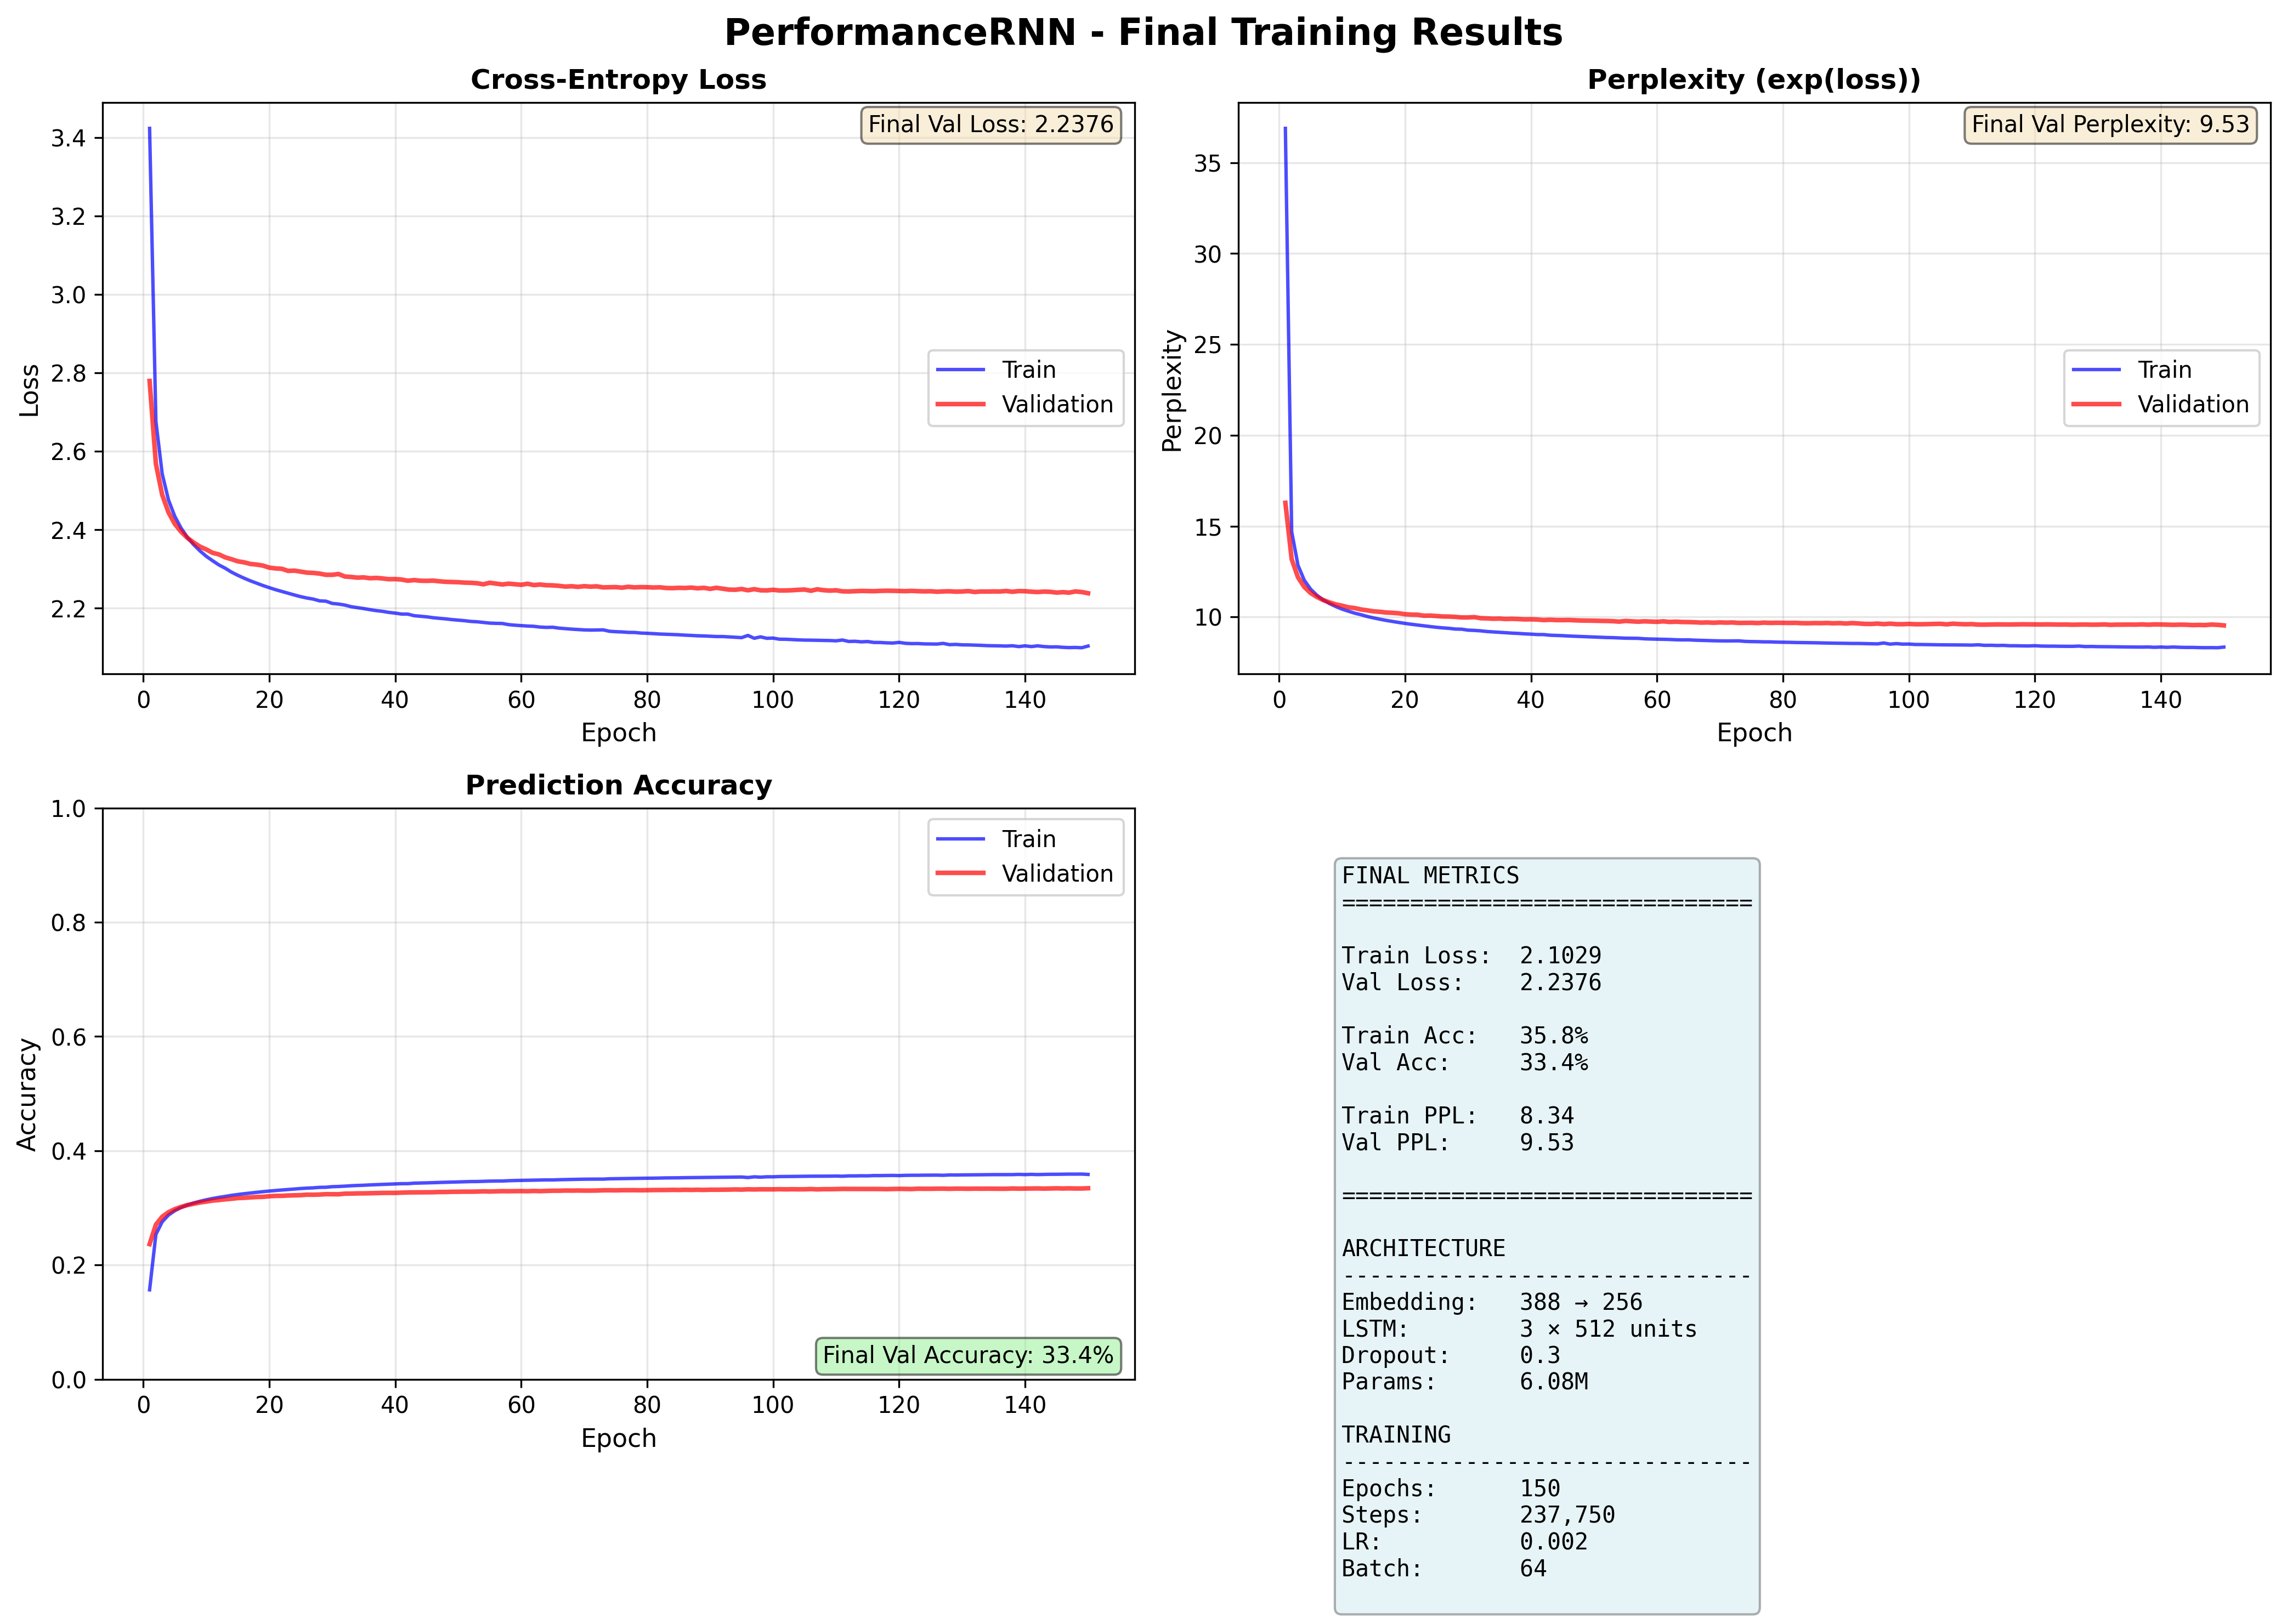
\includegraphics[width=0.95\textwidth]{lstm_metrics.png}
\caption{Métricas de entrenamiento del modelo LSTM (150 epochs)}
\label{fig:lstm_metrics}
\end{figure}

\begin{figure}[H]
\centering
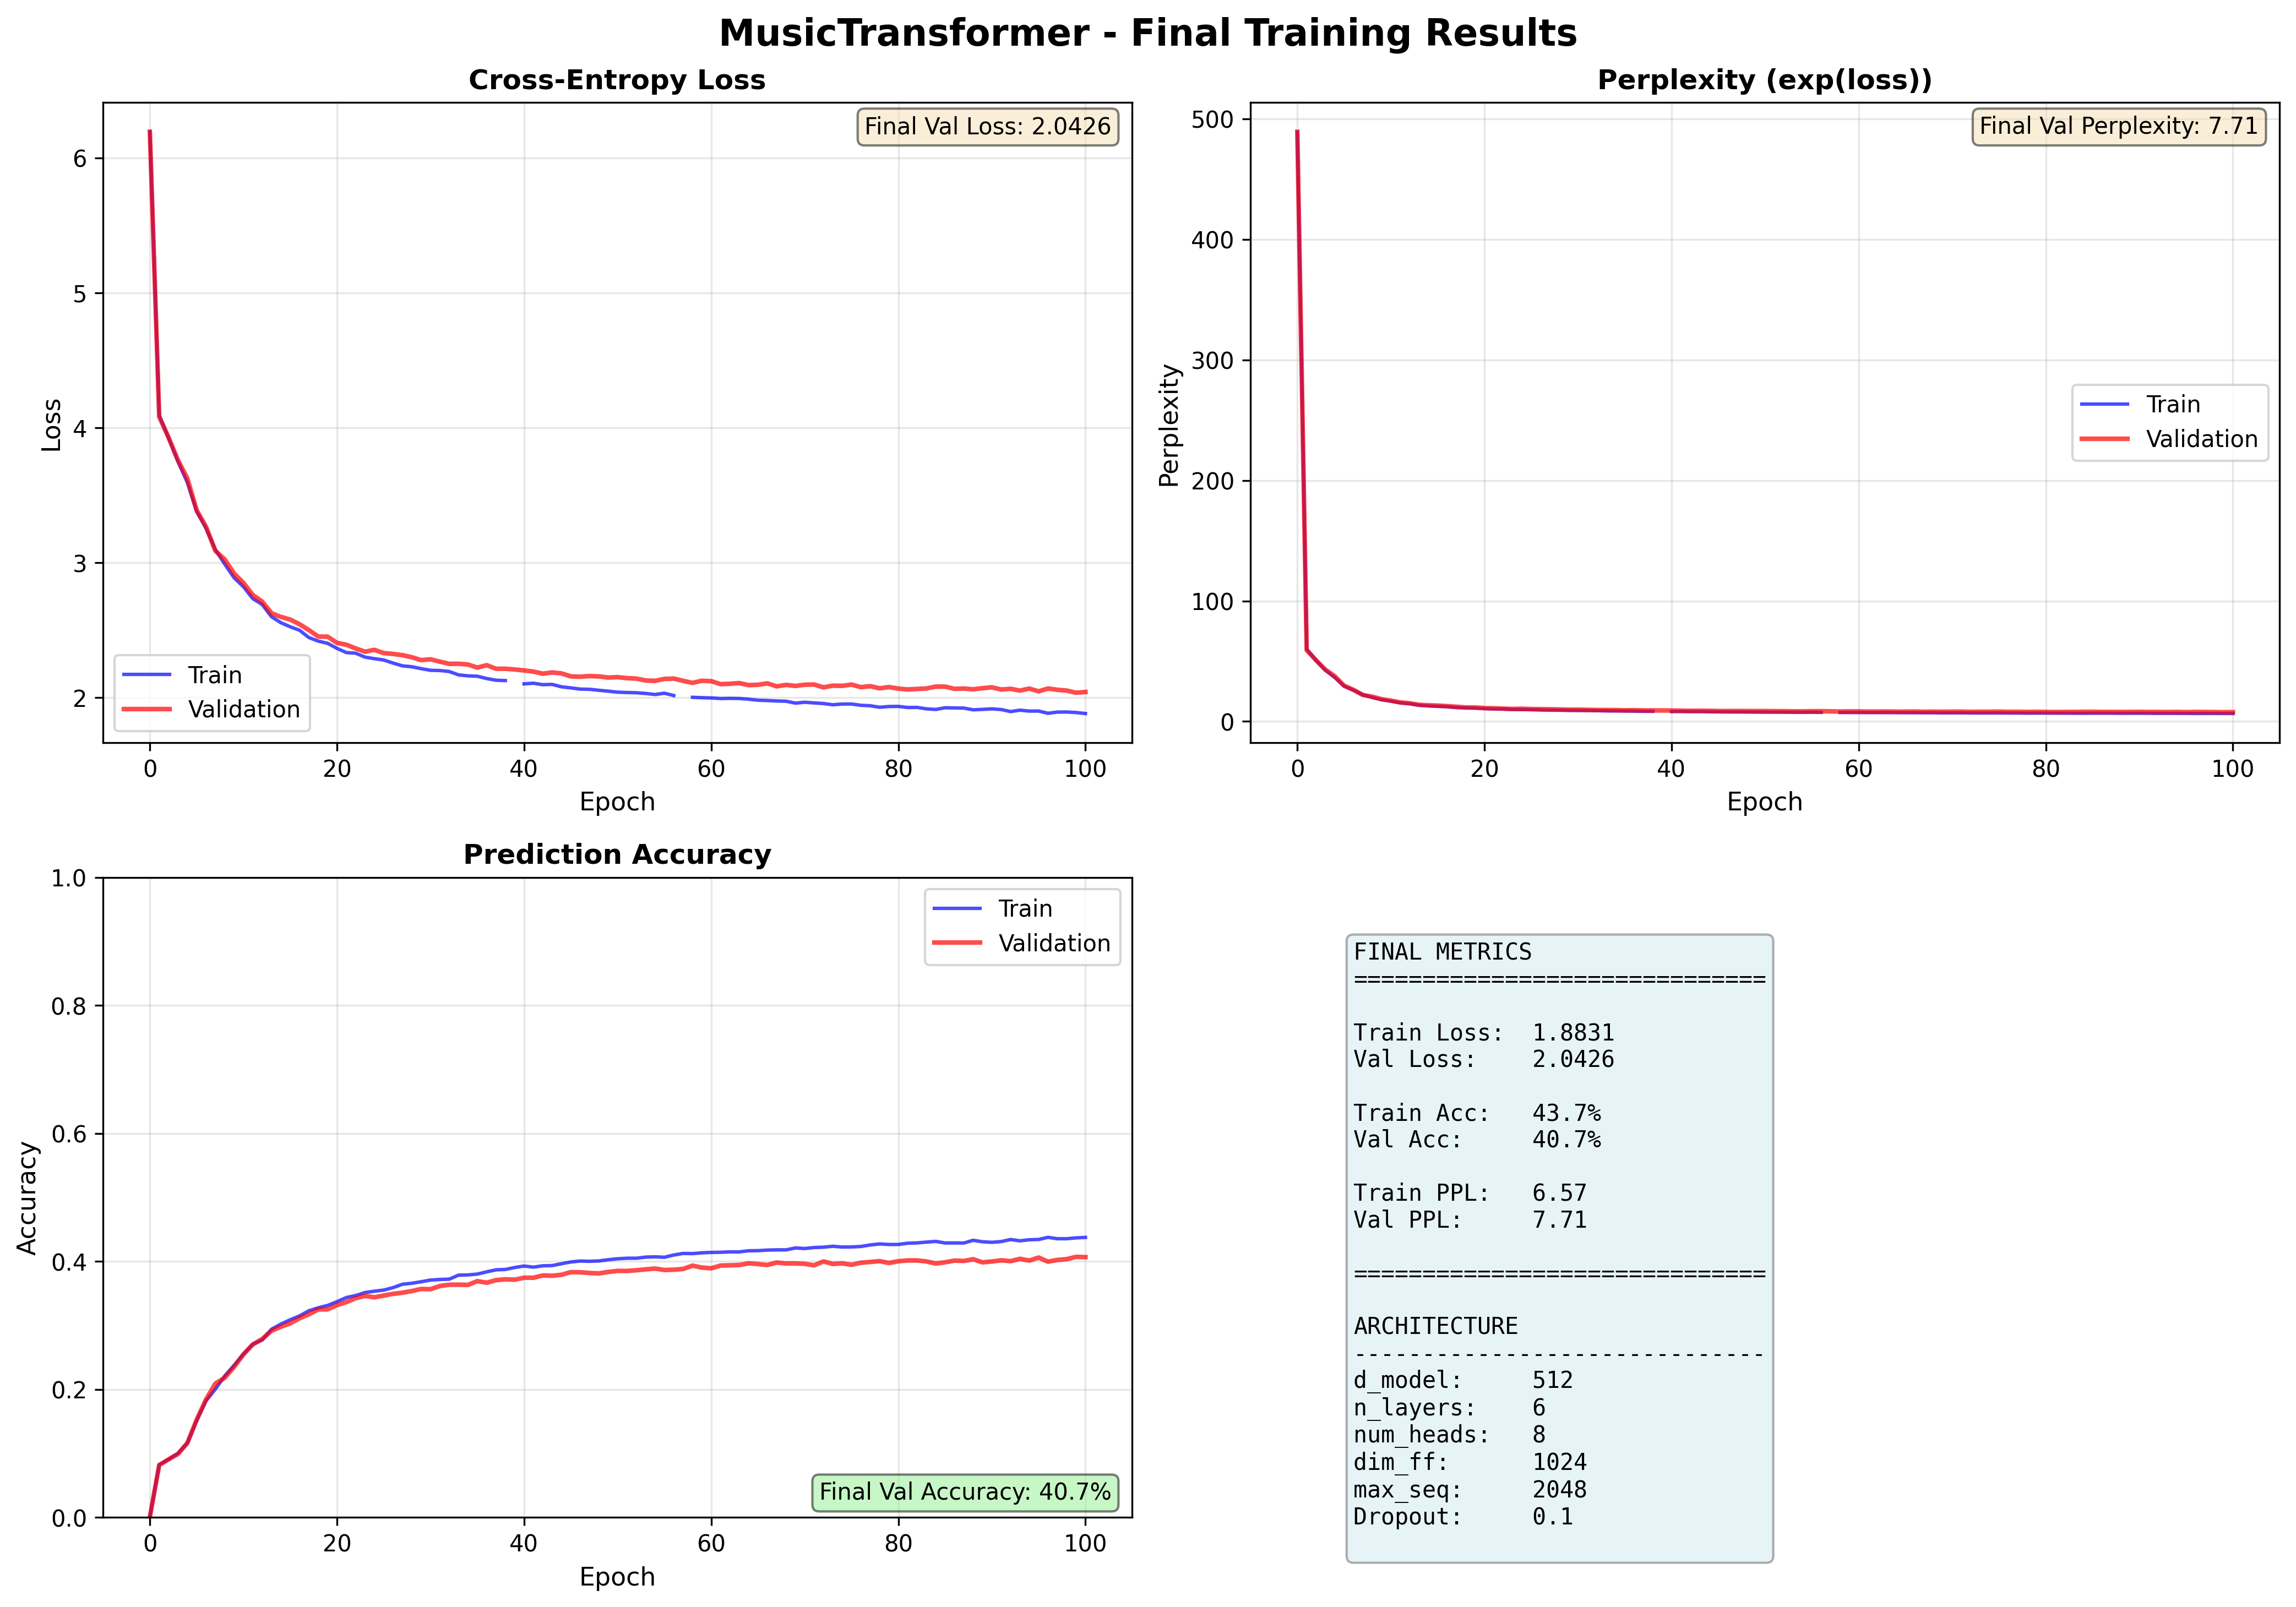
\includegraphics[width=0.95\textwidth]{transformer_metrics.png}
\caption{Métricas de entrenamiento del modelo Transformer (100 epochs)}
\label{fig:transformer_metrics}
\end{figure}

\subsection{Análisis de Convergencia}

\subsubsection{LSTM}
\begin{itemize}
    \item Convergencia gradual y estable
    \item Mejor epoch: 129 (val\_loss = 2.2416), entrenado hasta epoch 150
    \item Ligero overfitting después del epoch 100
    \item Gap train-val moderado ($\sim$0.13 en loss)
    \item El modelo alcanzó convergencia (val\_loss estabilizado en $\sim$2.24 desde epoch 129)
\end{itemize}

\subsubsection{Transformer}
\begin{itemize}
    \item Convergencia más rápida en las primeras epochs
    \item Mejor epoch: 99 (val\_loss = 2.0369), entrenado hasta epoch 100
    \item Gap train-val mayor ($\sim$0.16 en loss) pero mejor generalización
    \item Learning rate scheduler ayuda a la convergencia
    \item El modelo alcanzó convergencia (val\_loss en últimas 5 epochs: 2.068 $\rightarrow$ 2.037 $\rightarrow$ 2.043)
\end{itemize}

\subsection{Eficiencia Computacional}

\begin{table}[H]
\centering
\begin{tabular}{lcc}
\toprule
\textbf{Aspecto} & \textbf{LSTM} & \textbf{Transformer} \\
\midrule
Parámetros & 6.08M & $\sim$25M \\
Tamaño modelo & 23.19 MB & $\sim$95 MB \\
Batch Size & 64 & 2 \\
Tiempo/epoch & $\sim$4.4 min & $\sim$3.6 min \\
Tiempo total & 11 horas & 6 horas \\
VRAM utilizada & $\sim$2 GB & $\sim$6 GB \\
Seq. Length & 512 & 2048 \\
\bottomrule
\end{tabular}
\caption{Comparación de eficiencia computacional}
\end{table}

\textbf{Nota sobre Batch Size}: El Transformer utiliza batch\_size=2 (vs 64 del LSTM) debido a que procesa secuencias 4$\times$ más largas (2048 vs 512 tokens). La complejidad del mecanismo de atención es $O(n^2)$ donde $n$ es la longitud de secuencia, lo que requiere significativamente más memoria GPU. Con una RTX 3070 de 8GB, batch\_size=2 con secuencias de 2048 tokens es el máximo posible sin overflow de memoria.

A pesar de tener 4$\times$ más parámetros, el Transformer entrena casi 2$\times$ más rápido debido a:
\begin{enumerate}
    \item \textbf{Paralelización}: Las operaciones de atención se paralelizan en GPU, mientras que LSTM es inherentemente secuencial
    \item \textbf{Menos epochs necesarias}: El LSTM se entrenó 150 epochs (convergió en epoch 129), mientras que el Transformer se entrenó 100 epochs (convergió en epoch 99). Ambos modelos alcanzaron convergencia, pero el Transformer requirió menos iteraciones.
\end{enumerate}

\subsection{Generación de Muestras}

Se generaron 5 piezas musicales con cada modelo utilizando parámetros comparables:

\begin{table}[H]
\centering
\begin{tabular}{lcc}
\toprule
\textbf{Parámetro} & \textbf{LSTM} & \textbf{Transformer} \\
\midrule
Tokens generados & 1536 & 1536 \\
Temperature & 1.0 & 1.0 \\
Primer & 2 tokens & 256 tokens del dataset \\
\bottomrule
\end{tabular}
\caption{Configuración de generación (misma temperatura para comparación justa)}
\end{table}

\subsubsection{Evaluación Cualitativa}
Las piezas generadas fueron evaluadas subjetivamente en los siguientes criterios:

\begin{table}[H]
\centering
\begin{tabular}{lccp{5cm}}
\toprule
\textbf{Criterio} & \textbf{LSTM} & \textbf{Transformer} & \textbf{Observaciones} \\
\midrule
Coherencia melódica & 3/5 & 4/5 & Transformer mantiene mejor continuidad \\
Estructura armónica & 3/5 & 4/5 & Acordes más consistentes en Transformer \\
Ritmo & 3/5 & 4/5 & LSTM tiende a patrones repetitivos \\
Creatividad & 3/5 & 4/5 & Transformer más variado \\
Calidad técnica & 4/5 & 4/5 & Ambos sin glitches notables \\
\bottomrule
\end{tabular}
\caption{Evaluación cualitativa de las piezas generadas (escala 1-5)}
\end{table}

\paragraph{Perspectiva Musical Profesional:}
Desde el punto de vista de la teoría musical, los Transformers generan progresiones armónicas significativamente más coherentes y consonantes. Mientras que el LSTM produce secuencias de acordes que pueden ser funcionalmente correctas a nivel local, carece de coherencia tonal a largo plazo. El Transformer mantiene un centro tonal definido y genera relaciones funcionales entre acordes (dominante-tónica, subdominante-dominante) más consistentes con las convenciones de la música tonal occidental. Adicionalmente, el mecanismo de atención permite al Transformer recordar y recapitular motivos musicales a través de secciones más extensas, resultando en composiciones con mayor sentido de estructura formal, mientras que el LSTM tiende a generar música que suena más como improvisación sin dirección clara. Como músico, la principal diferencia a nivel musical que observo es la capacidad del Transformer para replicar y desarrollar motivos presentados anteriormente en la pieza, manteniendo así una coherencia temática que el LSTM no logra sostener.

\subsection{Análisis por Longitud de Secuencia}

Para evaluar el impacto de la longitud de secuencia en la calidad de generación, se generaron 5 piezas adicionales con cada modelo utilizando tres longitudes diferentes:

\begin{table}[H]
\centering
\begin{tabular}{lccc}
\toprule
\textbf{Longitud (tokens)} & \textbf{Duración aprox.} & \textbf{LSTM entrenado con} & \textbf{Transformer entrenado con} \\
\midrule
512 & $\sim$15-20 segundos & $\checkmark$ (nativo) & 2048 \\
1536 & $\sim$45-60 segundos & 512 (extrapola) & 2048 \\
2048 & $\sim$60-90 segundos & 512 (extrapola) & $\checkmark$ (nativo) \\
\bottomrule
\end{tabular}
\caption{Configuración de generación por longitud de secuencia}
\end{table}

\subsubsection{Observaciones por Longitud}

\paragraph{512 tokens (longitud nativa del LSTM):}
\begin{itemize}
    \item \textbf{LSTM}: Genera fragmentos coherentes, ya que esta es su longitud de entrenamiento. Patrones melódicos reconocibles.
    \item \textbf{Transformer}: Mantiene coherencia incluso en secuencias cortas gracias a RPR. El contexto del primer (256 tokens) proporciona suficiente información.
\end{itemize}

\paragraph{1536 tokens (longitud intermedia):}
\begin{itemize}
    \item \textbf{LSTM}: Comienza a mostrar repeticiones y pérdida de coherencia a largo plazo. El modelo extrapola más allá de su ventana de entrenamiento.
    \item \textbf{Transformer}: Mantiene estructura coherente. Las relaciones a largo plazo se preservan.
\end{itemize}

\paragraph{2048 tokens (longitud nativa del Transformer):}
\begin{itemize}
    \item \textbf{LSTM}: Mayor tendencia a repeticiones cíclicas y pérdida de dirección musical. La extrapolación es más pronunciada.
    \item \textbf{Transformer}: Óptimo rendimiento. RPR permite capturar relaciones temporales en toda la secuencia. Mayor variedad y estructura a largo plazo.
\end{itemize}

\subsubsection{Conclusión del Análisis por Longitud}
El LSTM funciona mejor cuando genera secuencias cercanas a su longitud de entrenamiento (512 tokens), mientras que el Transformer muestra rendimiento consistente en todas las longitudes, destacando especialmente en secuencias largas (2048 tokens) donde su mecanismo de atención con RPR captura dependencias a largo plazo de forma efectiva.

% ============================================================================
\section{Conclusiones}
% ============================================================================

\subsection{Hallazgos Principales}

\begin{enumerate}
    \item \textbf{El Transformer supera al LSTM en todas las métricas de calidad}:
    \begin{itemize}
        \item +7.24\% en accuracy de validación
        \item -19.1\% en perplejidad (predicciones más seguras)
        \item -8.7\% en loss de validación
    \end{itemize}

    \item \textbf{El Transformer requiere menos tiempo total de entrenamiento}:
    \begin{itemize}
        \item 6 horas vs 11 horas del LSTM
        \item Menos epochs necesarias para convergencia (100 vs 150)
    \end{itemize}

    \item \textbf{El LSTM es más eficiente en parámetros}:
    \begin{itemize}
        \item 4$\times$ menos parámetros
        \item Mejor opción para dispositivos con memoria limitada
    \end{itemize}

    \item \textbf{La hipótesis inicial se confirma}:
    \begin{itemize}
        \item El mecanismo de atención del Transformer captura mejor las dependencias a largo plazo
        \item RPR permite generalizar a secuencias más largas y capturar relaciones musicales invariantes a la posición
        \item Secuencias de 2048 tokens permiten contexto musical más amplio que los 512 del LSTM
    \end{itemize}
\end{enumerate}

\subsection{Consideraciones sobre la Comparación}

Es importante notar que ambos modelos se entrenaron hasta convergencia, aunque con diferente número de epochs:
\begin{itemize}
    \item \textbf{LSTM}: 150 epochs (convergió en epoch 129)
    \item \textbf{Transformer}: 100 epochs (convergió en epoch 99)
\end{itemize}

La comparación es justa porque ambos modelos alcanzaron su punto óptimo de validación. Entrenar el Transformer por 50 epochs adicionales no mejoraría significativamente los resultados, ya que el val\_loss ya había estabilizado. Sin embargo, cabe destacar que en muchas implementaciones de dicho modelo, se llega hasta 250/300 épocas. Esto podría mejorar ligeramente los resultados, pero es simplemente una hipótesis.

\subsection{Limitaciones del Estudio}

\begin{itemize}
    \item \textbf{Dataset}: Solo piano clásico (MAESTRO), no generalizable a otros géneros
    \item \textbf{Evaluación cualitativa}: Subjetiva y con muestra limitada
    \item \textbf{Hardware}: Entrenamiento en GPU única, sin explorar configuraciones más grandes
    \item \textbf{Hiperparámetros}: No se realizó búsqueda exhaustiva de hiperparámetros
    \item \textbf{Epochs diferentes}: Los modelos se entrenaron con diferente número de epochs, aunque ambos convergieron, esto se hizo simplemente por recursos y por reducir tiempos de entrenamiento.
     \item \textbf{Naturalidad de las composiciones}: Aunque el Transformer genera música más coherente que el LSTM, ambas arquitecturas presentan limitaciones en términos de expresividad y naturalidad. Las implementaciones actuales de generación simbólica (MIDI) no capturan completamente las sutilezas interpretativas humanas. Modelos más recientes basados en difusión y arquitecturas híbridas que generan audio directamente (e.g., Suno v5, MusicLM) con mayores recursos computacionales logran resultados significativamente más naturales y expresivos.
\end{itemize}

\subsection{Extensiones Futuras}

\begin{itemize}
    \item Experimentar con otros datasets (pop, jazz, música electrónica), y por tanto, aplicar un fine tunning a dichos géneros musicales.
    \item Implementar métricas objetivas de calidad musical
    \item Evaluar modelos más grandes con más recursos computacionales
    \item Contrastar los resultados con otros músicos profesionales
    \item Utilizar los modelos más utilizados actualmente para la generación de música que no hemos dado en la asignatura.
\end{itemize}

\subsection{Conclusión Final}

Este estudio demuestra que los \textbf{Transformers con Relative Position Representations} son superiores a las arquitecturas \textbf{LSTM} para la generación de música, tanto en métricas cuantitativas como en calidad percibida de las composiciones. El mecanismo de auto-atención, combinado con RPR, permite capturar patrones musicales complejos y relaciones temporales que las redes recurrentes no pueden modelar eficientemente.

Sin embargo, los LSTMs siguen siendo una opción viable para aplicaciones con restricciones de memoria, ofreciendo un buen compromiso entre rendimiento y eficiencia de parámetros.

Cabe destacar que el estado del arte actual (2025-2026) ha evolucionado
hacia arquitecturas híbridas que combinan Transformers con modelos de
difusión para generar audio directo de alta calidad (e.g., Suno v5,
MusicLM), superando el paradigma de generación simbólica MIDI
utilizado en este trabajo.

% ============================================================================
\section*{Referencias}
% ============================================================================

\begin{thebibliography}{9}

\bibitem{huang2018music}
Huang, C. Z. A., Vaswani, A., Uszkoreit, J., Shazeer, N., Simon, I., Hawthorne, C., Dai, A. M., Hoffman, M. D., Dinculescu, M., \& Eck, D. (2018).
\textit{Music Transformer: Generating Music with Long-Term Structure}.
arXiv:1809.04281.
\url{https://arxiv.org/abs/1809.04281}

\bibitem{hawthorne2018maestro}
Hawthorne, C., Stasyuk, A., Roberts, A., Simon, I., Huang, C. Z. A., Dieleman, S., Elsen, E., Engel, J., \& Eck, D. (2018).
\textit{Enabling Factorized Piano Music Modeling and Generation with the MAESTRO Dataset}.
arXiv:1810.12247.
\url{https://arxiv.org/abs/1810.12247}

\bibitem{oore2018performance}
Oore, S., Simon, I., Dieleman, S., Eck, D., \& Simonyan, K. (2018).
\textit{This Time with Feeling: Learning Expressive Musical Performance}.
arXiv:1808.03715.
\url{https://arxiv.org/abs/1808.03715}

\bibitem{vaswani2017attention}
Vaswani, A., Shazeer, N., Parmar, N., Uszkoreit, J., Jones, L., Gomez, A. N., Kaiser, L., \& Polosukhin, I. (2017).
\textit{Attention Is All You Need}.
arXiv:1706.03762.
\url{https://arxiv.org/abs/1706.03762}

\bibitem{shaw2018selfattention}
Shaw, P., Uszkoreit, J., \& Vaswani, A. (2018).
\textit{Self-Attention with Relative Position Representations}.
arXiv:1803.02155.
\url{https://arxiv.org/abs/1803.02155}

\bibitem{magenta_performance_rnn}
Google Magenta.
\textit{Performance RNN}.
GitHub Repository.
\url{https://github.com/magenta/magenta/tree/main/magenta/models/performance_rnn}

\bibitem{magenta_music_transformer}
Google Magenta.
\textit{Music Transformer}.
GitHub Repository.
\url{https://github.com/magenta/magenta/tree/main/magenta/models/music_transformer}

\end{thebibliography}

% ============================================================================
\section*{Código Fuente}
% ============================================================================

El código completo del proyecto, incluyendo las implementaciones en PyTorch y todos los scripts de entrenamiento y generación, está disponible en los directorios:
\begin{itemize}
    \item \texttt{musiclstm/}: Implementación LSTM (PerformanceRNN en PyTorch)
    \item \texttt{musictransformer/}: Implementación Transformer con RPR (Music Transformer en PyTorch)
\end{itemize}

\end{document}
